\chapter{Modellazione dei Casi d'Uso}
\section{Attori e Casi d'Uso}
\begin{table}[!hbp]
	\centering
	\begin{tblr}{colspec=XX}
		\begin{minipage}[t]{\linewidth}
			\paragraph{Attori primari}
			\begin{itemize}
				\item Utente
				\item UtenteAutenticato
				\item Amministratore
			\end{itemize}
		\end{minipage} &
		\begin{minipage}[t]{\linewidth}
			\paragraph{Attori secondari}
			\begin{itemize}
				\item Sistema Bancario
			\end{itemize}
		\end{minipage} \\
	\end{tblr}
\end{table}
\begin{table}[!hbp]
	\centering
	\begin{tblr}{colspec=XX}
		\begin{minipage}[t]{\linewidth}
			\paragraph{Casi d'uso}
			\begin{enumerate}
				\item Registrazione 
				\item VisualizzaProfiloPersonale
				\item ModificaDatiPersonali
				\item VisualizzaBiglietto
				\item ScaricaBiglietto
				\item RichiediCatalogoEventi
				\item FiltraCatalogo
				\item AcquistoBiglietto
				\item VisualizzaElencoEventiOdierni
				\item PartecipazioneEvento
			\end{enumerate}
		\end{minipage} &
		\begin{minipage}[t]{\linewidth}
			\paragraph{Casi d'uso di inclusione}
			\begin{enumerate}
                \item VisualizzaProfiloPersonale
                \item RichiediCatalogoEventi
                \item VisualizzaElencoEventiOdierni
			\end{enumerate}
			\paragraph{Casi d'uso di estensione}
			\begin{enumerate}
				\item FiltraCatalogo
			\end{enumerate}
		\end{minipage}
	\end{tblr}
\end{table}
\begin{table}[!ht]
\centering
\small
\begin{tblr}{
  colspec = {X[2,l] X[1.2,l] X[1,l] X[1.6,l] X[1.5,l]},
  hlines,
  row{1} = {font=\bfseries}
}
Caso d'uso & Attori Primari & Attori Secondari & Incl. / Ext. & Requisiti corrispondenti \\
Registrazione & Utente & -- & -- & \Req{rf}{01} \\
AccessoProfiloPersonale & Utente Autenticato & --  & -- &\Req{rf}{04} \\
ConsultaCatalogoEventi & Utente Autenticato & -- & -- &\Req{rf}{07} \\
ConsultaElencoEventiOdierni & Utente Autenticato & --  &--& \Req{rf}{13} \\
Aggiugni Evento & Amministratore & -- & -- & \Req{rf}{06} \\
Visualizza Informazioni Evento & Amministratore & -- & -- & \Req{rf}{17}, \Req{rf}{18} \\
Filtra Catalogo & -- & -- & Include: Consulta Catalogo Eventi & \Req{rf}{08} \\
Modifica Dati Personali & Utente Autenticato & -- & Include: Accesso Profilo Personale & \Req{rf}{05} \\
Visualizza Biglietto & Utente Autenticato & -- & Include: Accesso Profilo Personale & \Req{rf}{11} \\
Scarica Biglietto & Utente Autenticato & -- & Include: Accesso Profilo Personale & \Req{rf}{12} \\
Acquisto Biglietto & Utente Autenticato & Sistema Gestione Acquisti & Include: Consulta Catalogo Eventi & \Req{rf}{09}, \Req{rf}{10} \\
Partecipazione Evento & Utente Autenticato & -- & Include: Consulta Elenco Eventi Odierni & \Req{rf}{14} \\
\end{tblr}
\end{table}

\section{Diagramma dei Casi d'Uso}
\begin{table}[!ht]
\centering
	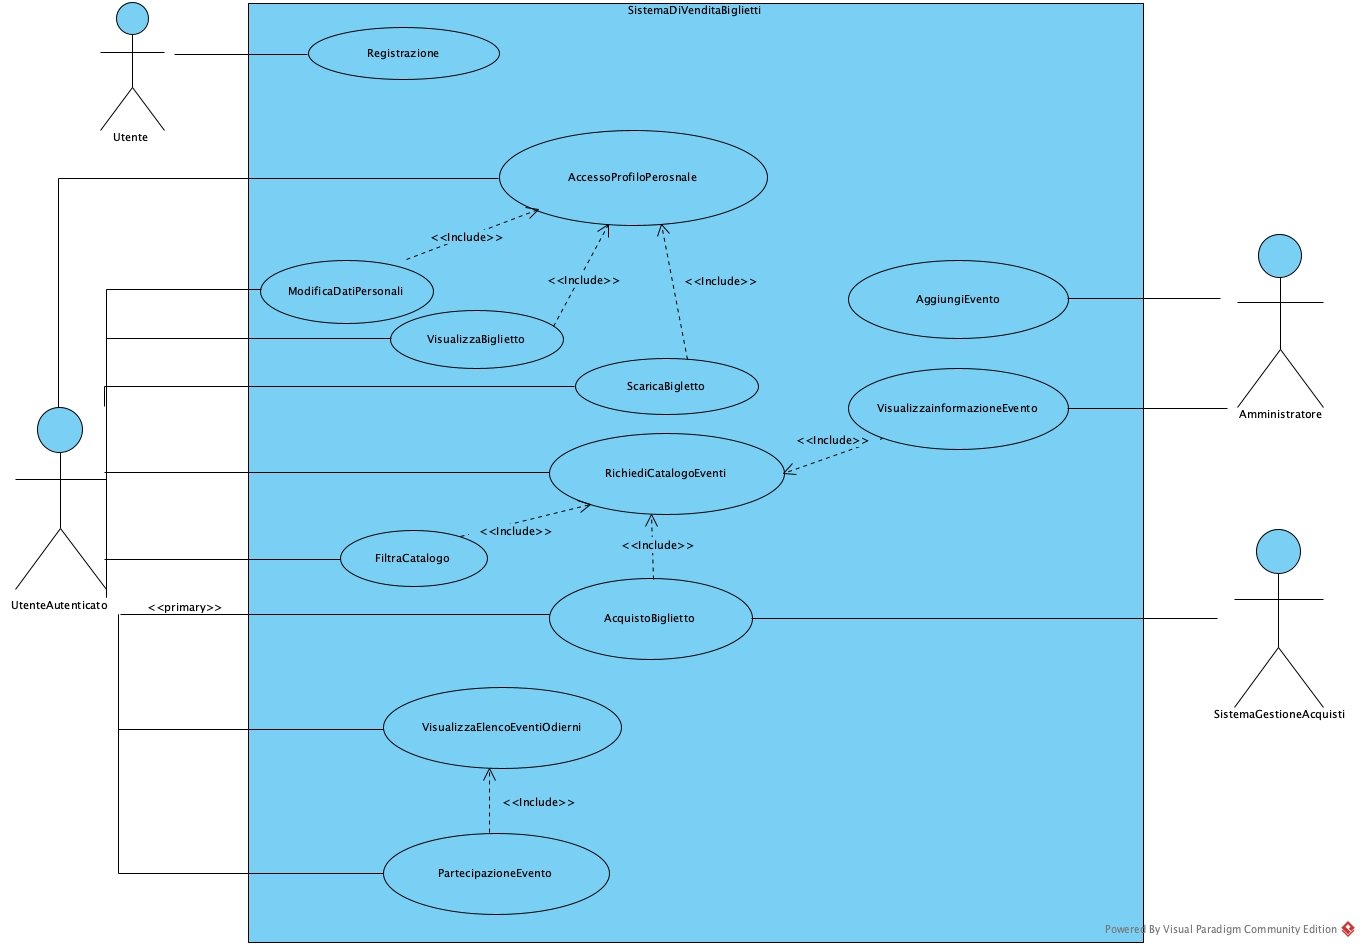
\includegraphics[width=\linewidth]{assets/usd.jpg}
\end{table}	
\pagebreak
\section{Scenari}
\IncludeTable{capitoli/scenari/Registrazione}
\IncludeTable{capitoli/scenari/VisualizzaProfiloPersonale}
\IncludeTable{capitoli/scenari/ModificaDatiPersonali}
\IncludeTable{capitoli/scenari/RichiediCatalogoEventi}
\IncludeTable{capitoli/scenari/FiltraCatalogo}
\IncludeTable{capitoli/scenari/VisualizzaElencoEventiOdierni}
\IncludeTable{capitoli/scenari/ScaricaBiglietto}
\IncludeTable{capitoli/scenari/VisualizzaBiglietto}
\IncludeTable{capitoli/scenari/AcquistaBiglietto}
\IncludeTable{capitoli/scenari/CreazioneEvento}
\IncludeTable{capitoli/scenari/PartecipazioneEvento}

\IncludeTable{capitoli/scenari/VisualizzaInformazioniEvento}